\testfile{pgfplotstest.marks.tex}
{
	%\tracingmacros=2\tracingcommands=2
	\def\smallplotstest{%
	\addplot coordinates {
		(-1,	1)
		(-0.75,	0.5625)
		(-0.5,	0.25)
		(-0.25,	0.0625)
		(0,		0)
		(0.25,	0.0625)
		(0.5,	0.25)
		(0.75,	0.5625)
		(1,		1)
	};
	}
	\testsection{Testing special treatment for no marks and only marks}
	\testsubsection{both, marks and lines}
	\testsubsubsection{Normal plot}
	\begin{tikzpicture}
		\begin{axis}
			\smallplotstest
		\end{axis}
	\end{tikzpicture}

	\testsubsubsection{log plot}
	\begin{tikzpicture}
		\begin{loglogaxis}
			\loglogtestplot
		\end{loglogaxis}
	\end{tikzpicture}

	\testsubsection{only marks}
	{\pgfplotsset{cycle list={{blue,only marks,mark=*},{red,only marks,mark=x}}}
	\testsubsubsection{Normal plot}
	\begin{tikzpicture}
		\begin{axis}
			\smallplotstest
		\end{axis}
	\end{tikzpicture}

	\testsubsubsection{log plot}
	\begin{tikzpicture}
		\begin{loglogaxis}
			\loglogtestplot
		\end{loglogaxis}
	\end{tikzpicture}
	}

	\testsubsection{no marks}
	{\pgfplotsset{cycle list={{blue},{red}}}
	\testsubsubsection{Normal plot}
	\begin{tikzpicture}
		\begin{axis}
			\smallplotstest
		\end{axis}
	\end{tikzpicture}

	\testsubsubsection{log plot}
	\begin{tikzpicture}
		\begin{loglogaxis}
			\loglogtestplot
		\end{loglogaxis}
	\end{tikzpicture}
	}




	\testsection{Testing special treatment for no marks and only marks for STACKED PLOTS}
	{
		%\tracingmacros=2\tracingcommands=2
		\pgfplotsset{stack plots=y}
		\def\smallplotstest{%
			\addplot coordinates {(0,1) (1,2) (2,2) (3,4)};
			\addplot coordinates {(0,1) (1,2) (2,2) (3,4)};
		}
		\def\loglogtestplot{%
			\addplot coordinates {(1e3,1e-4) (1e4,1e-5) (1e5,1e-5) (1e6,1e-6)};
			\addplot coordinates {(1e3,1e-4) (1e4,1e-5) (1e5,1e-5) (1e6,1e-6)};
		}%
		\testsubsection{both, marks and lines}
		\testsubsubsection{Normal plot}
		\begin{tikzpicture}
		%\tracingmacros=2\tracingcommands=2
			\begin{axis}
				\smallplotstest
			\end{axis}
		\end{tikzpicture}

		\testsubsubsection{log plot}
		\begin{tikzpicture}
		%\tracingmacros=2\tracingcommands=2
			\begin{loglogaxis}
				\loglogtestplot
			\end{loglogaxis}
		\end{tikzpicture}

		\testsubsection{only marks}
		{
		\pgfplotsset{cycle list={{blue,only marks,mark=*},{red,only marks,mark=x}}}
		\testsubsubsection{Normal plot}
		\begin{tikzpicture}
			\begin{axis}
				\smallplotstest
			\end{axis}
		\end{tikzpicture}

		\testsubsubsection{log plot}
		\begin{tikzpicture}
			\begin{loglogaxis}
				\loglogtestplot
			\end{loglogaxis}
		\end{tikzpicture}
		}

		\testsubsection{no marks}
		{
		\pgfplotsset{cycle list={{blue},{red}}}
		\testsubsubsection{Normal plot}
		\begin{tikzpicture}
			\begin{axis}
				\smallplotstest
			\end{axis}
		\end{tikzpicture}

		\testsubsubsection{log plot}
		\begin{tikzpicture}
			\begin{loglogaxis}
				\loglogtestplot
			\end{loglogaxis}
		\end{tikzpicture}
		}
	}

	\testsection{nodes near coords}
	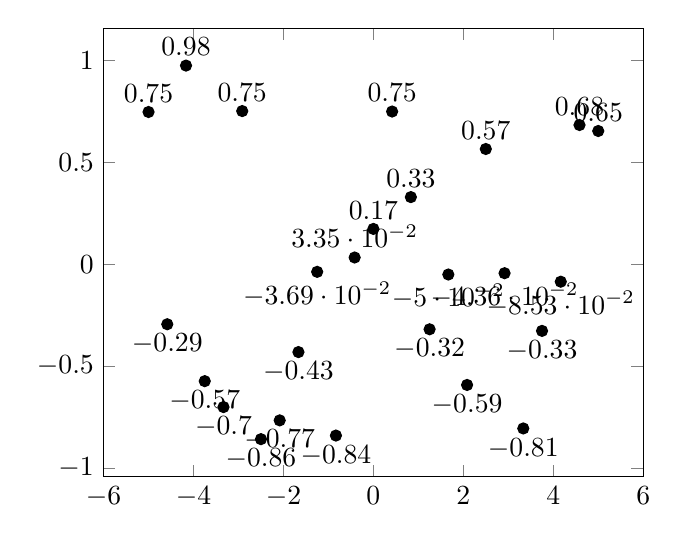
\begin{tikzpicture}
	%\tracingcommands=2\tracingmacros=2
		\begin{axis}[nodes near coords]
		\addplot[scatter,only marks] {rand};	
		\end{axis}
	\end{tikzpicture}

	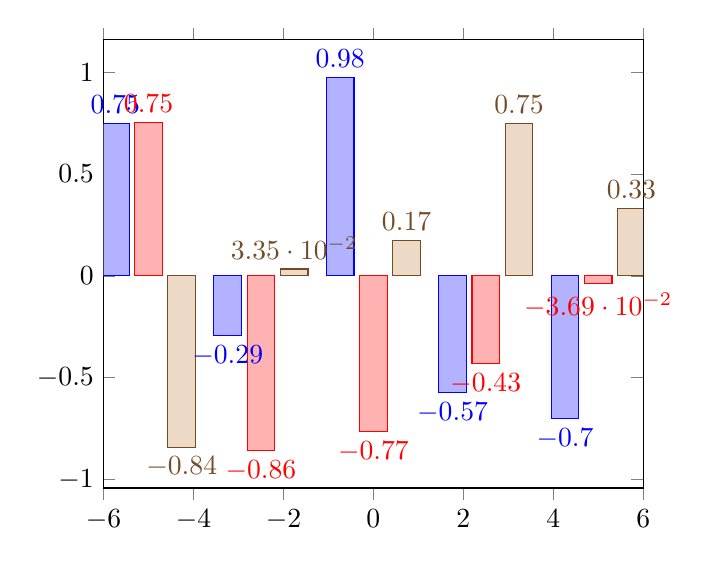
\begin{tikzpicture}
	%\tracingcommands=2\tracingmacros=2
		\begin{axis}[nodes near coords,ybar,samples=5]
		\addplot {rand};	
		\addplot {rand};	
		\addplot {rand};	
		\end{axis}
	\end{tikzpicture}

	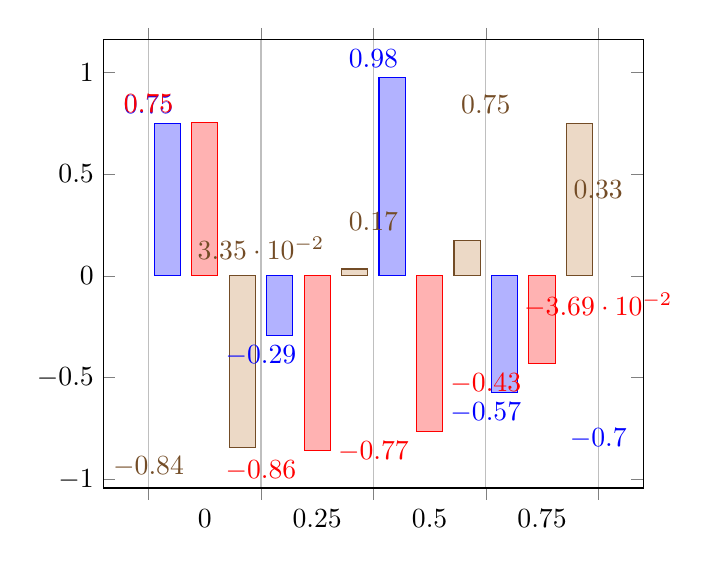
\begin{tikzpicture}
	%\tracingcommands=2\tracingmacros=2
		\begin{axis}[nodes near coords,ybar interval=0.7,samples=5,domain=0:1]
		\addplot {rand};	
		\addplot {rand};	
		\addplot {rand};	
		\end{axis}
	\end{tikzpicture}

	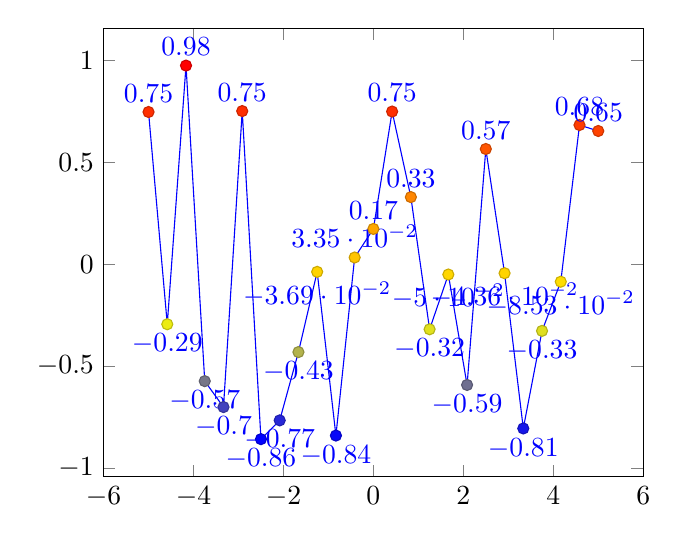
\begin{tikzpicture}
	%\tracingcommands=2\tracingmacros=2
		\begin{axis}[nodes near coords*]
		\addplot {rand};	
		\end{axis}
	\end{tikzpicture}

}
